\documentclass{article}
\usepackage{verbatim}
\usepackage{amsmath}
\usepackage{pdfpages}
\usepackage{xeCJK}
\usepackage{hyperref}
\usepackage{listings}
\lstset{
 columns=fixed,       
 numbers=left,                                        % 在左侧显示行号
 numberstyle=\tiny\color{gray},                       % 设定行号格式
 frame=single,                                          % 不显示背景边框
 keywordstyle=\color[RGB]{40,40,255},                 % 设定关键字颜色
 numberstyle=\footnotesize\color{darkgray},           
 commentstyle=\it\color[RGB]{0,96,96},                % 设置代码注释的格式
 stringstyle=\rmfamily\slshape\color[RGB]{128,0,0},   % 设置字符串格式
 showstringspaces=false,                              % 不显示字符串中的空格
 language=c++,                                        % 设置语言
}
\newcommand{\paper}[2]{\hyperlink{./papers/#1.pdf.#2}{(P#2)}}
\newcommand{\book}[2]{\href[page=#2]{./books/#1.pdf}{(P#2)}}


\title{Near-Data Processing}
\author{陈辉}
\date{}
\begin{document}
\maketitle
\tableofcontents
\newpage
\part{文献}
\section{\textit{Cloud-Scale-Acceleration-Architecture}}
\paper{Cloud-Scale-Acceleration-Architecture}{1}
\subsection{Introduction}
\textbf{Balance of Homogeneity and Specialization}\par
Specialized accelerator should be programmable to adjust the diversity of cloud servers and rapid change. That's why we need FPGAs or GPUs.\\

This paper describes a cloud-scale FPGA-based acceleration architecture called \textit{Configurable Cloud} which allows datapath of cloud communication to be accelerated with FPGAs. This datapath can include networking flows, \textbf{storage flows}, security operations and distributed applications.\\

We use a protocol called \textbf{LTL(Lightweight Transport Layer)} to make the remote FPGA resources apper closer than either a single local SSD access or the time to get through the host's networking stack.\\

\subsection{Hardware Architecture}
\textbf{Designing Requirements}
\begin{itemize}
\item Homogeneity.
\item Fungibility.
\item Flexibility.

\begin{itemize}
\item \textit{Local compute acceleration(through PCIe)}.
Local acceleration handles \textbf{hight-value scenarios} such as search rankingon each FPGA's host. 
\item \textit{Network acceleration.} 
e.g. intrusion detection, deep packet inspection and network encryption.
\item \textit{Global application acceleration(through FPGA pools)}. Through this, idle FPGAs can be used for distributed large-scale applications such as machine learning.
\end{itemize}

\item \textbf{Physical restrictions}. e.g. physical space, power consumption, and temperature. That's \textbf{why we choose FPGAs instead of GPUs}.
\end{itemize}





\section{\textit{Practical-Near-Data-Processing-for-In-memory-Analytics-Frameworks}}
See paper\paper{Practical-Near-Data-Processing-for-In-memory-Analytics-Frameworks}{1}
See presentation\paper{Practical-Near-Data-Processing-for-In-memory-Analytics-Frameworks(Presentation)}{1}






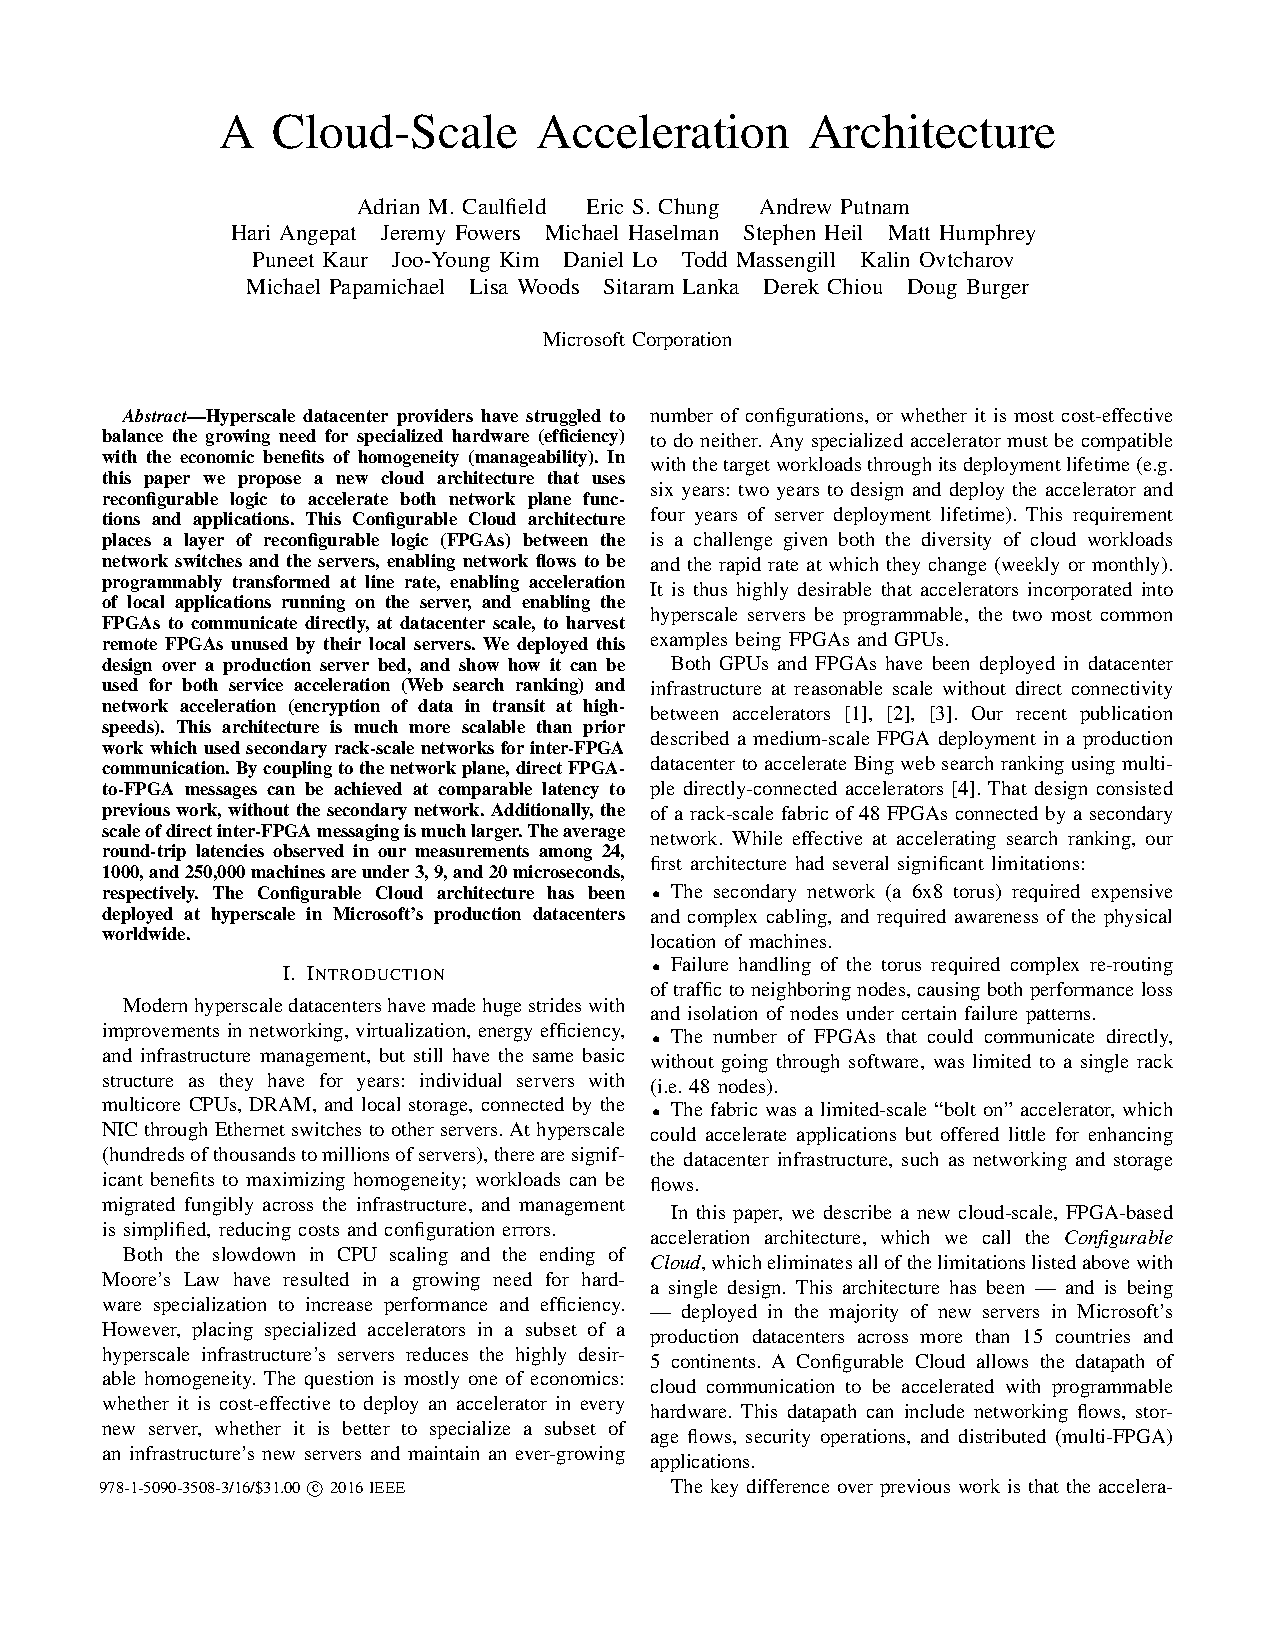
\includepdf[link=true,pages=-,fitpaper]{./papers/Cloud-Scale-Acceleration-Architecture.pdf}
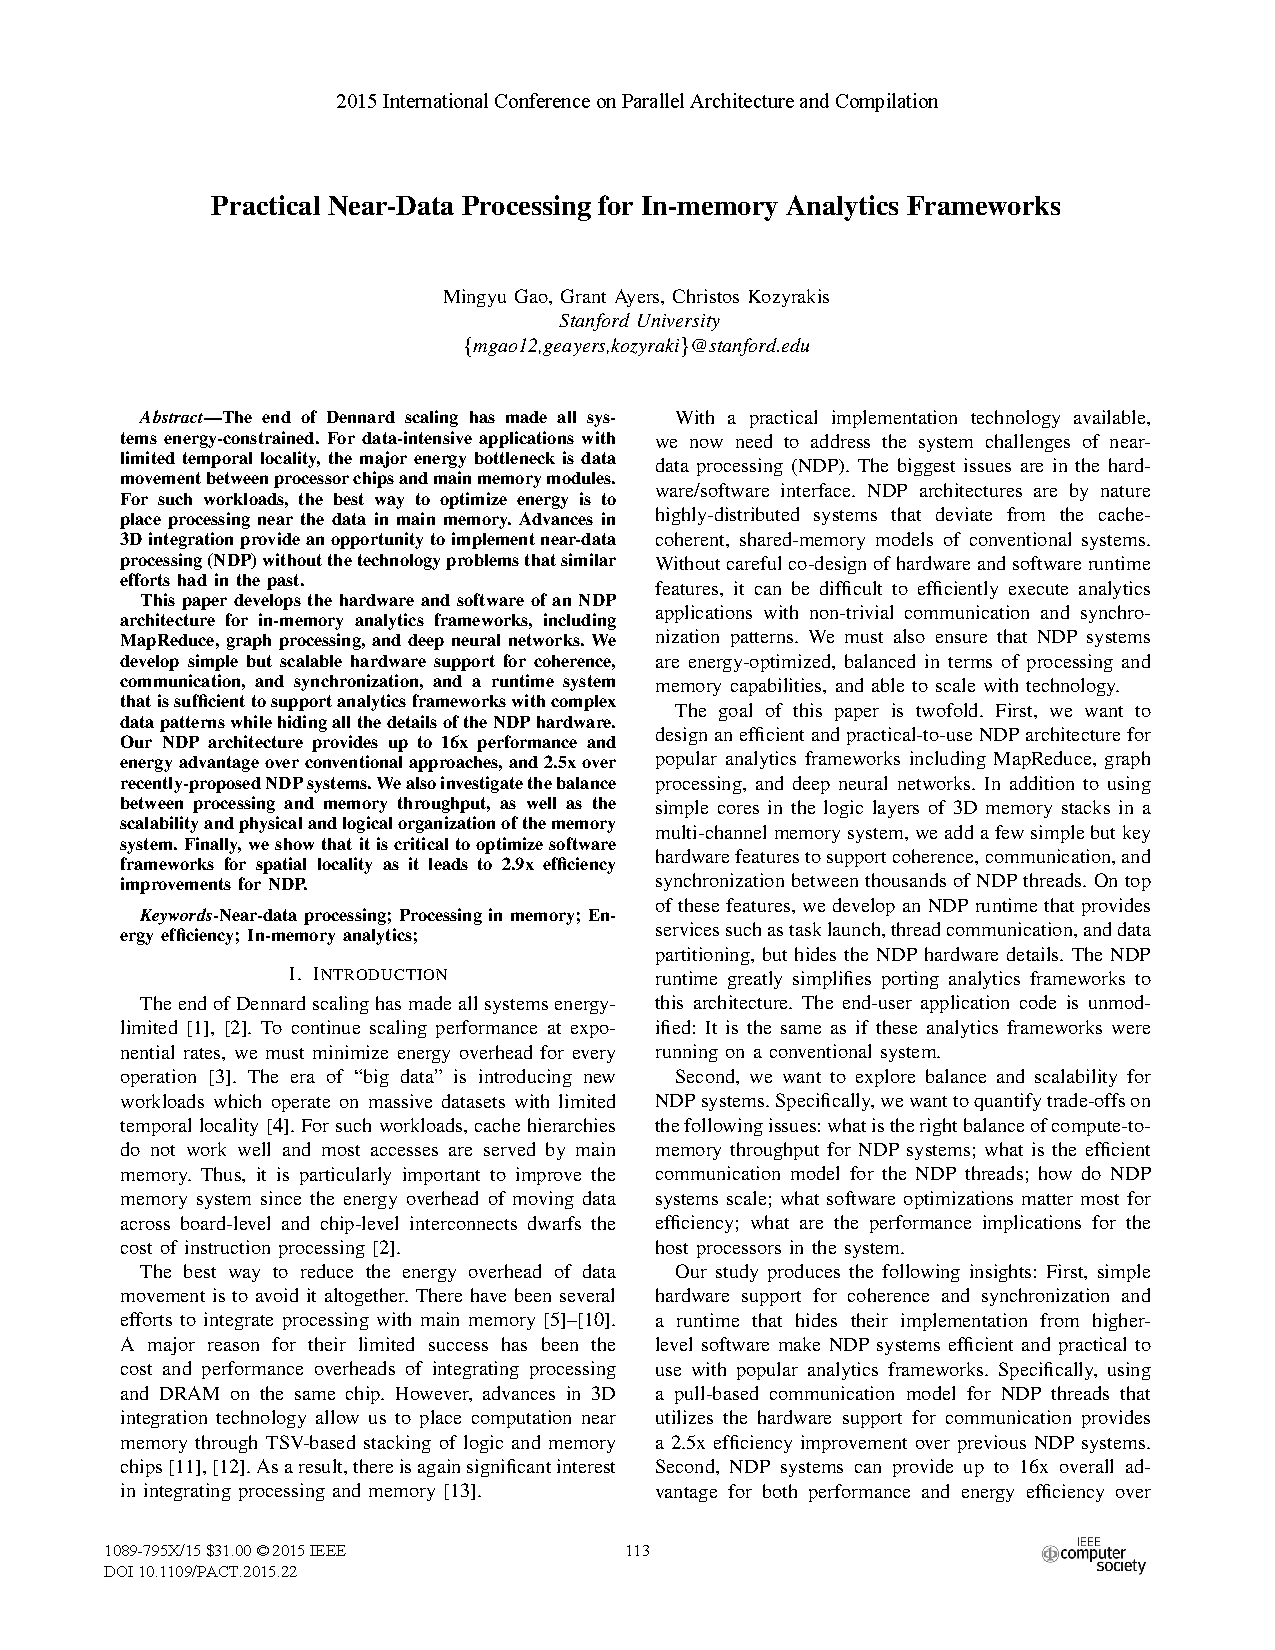
\includepdf[link=true,pages=-,fitpaper]{./papers/Practical-Near-Data-Processing-for-In-memory-Analytics-Frameworks.pdf}
%\includepdf[link=true,pages=-,fitpaper]{./papers/<++>.pdf}
%\includepdf[link=true,pages=-,fitpaper,angle=-90]{./papers/<++>.pdf}

\end{document}
